\documentclass[main.tex]{subfiles}
\begin{document}

\section{Sheet 7}

\subsection{Photons travelling in the Schwarzschild metric}

\subsubsection{A different proof for the conservation of the component of the velocity of a geodesic along a Killing vector field (complement)}

Here I present a different proof to what was done in the lectures for the fact that the component of the 4-velocity along the Killing vector field is conserved. 
This is not necessary to know for the exam, do skip this section if it does not interest you. 

If the metric does not depend on the coordinate \(\widetilde{\alpha }\), then \(\partial_{\widetilde{\alpha }} g_{\mu \nu } = 0\). So, let us differentiate covariantly the vector \(\xi_{\mu } = g_{\mu \nu } \delta^{\nu}_{\widetilde{\alpha }}\).
It will be apparent later that differentiating the lower-index vector field gives us the interesting property.
We get 
%
\begin{align}
  \nabla_{\mu } \xi_{\nu } =
  g_{\nu \sigma } \nabla_{\mu } \xi^{\sigma }
  =  g_{\nu \sigma }
  \qty(\cancelto{}{\partial_{\mu } \xi^{\sigma }} + \Gamma^{\sigma }_{\mu \rho } \xi^{\rho })
  = \Gamma_{\nu \mu \widetilde{\alpha }}
\,,
\end{align}
%
since the only component which survives the contraction with \(\xi \) is the one along \(\widetilde{\alpha} \); also, we lowered an index of the Christoffel symbols with the metric. 

The explicit expression for the lower indices Christoffel symbols is 
%
\begin{align}
  \Gamma_{\nu \mu \widetilde{\alpha }}
  = \frac{1}{2} \qty(\cancelto{}{g_{\mu \nu , \widetilde{\alpha }}} +
  g_{\mu \widetilde{\alpha }, \nu }
  - g_{\mu \widetilde{\alpha }, \nu })
\,,
\end{align}
%
since by hypothesis any derivative of the metric along \(\widetilde{\alpha}\) is zero. So, we can directly see that the object \(\nabla_{\mu } \xi_{\nu }\) is antisymmetric in its indices: this can be written as 
%
\begin{align}
  \nabla_{(\mu } \xi_{\nu )} = 0
\,,
\end{align}
%
and is called \emph{Killing's equation}. We have shown that is equivalent to the metric not depending on the coordinate \(x^{\widetilde{\alpha}}\).

Now, we can quickly prove the conservation a component of the 4-velocity of a geodesic along the Killing vector field: we just need to differentiate \(u^{\mu } \xi_{\mu }\) with respect to the arc parameter. 
Recall that geodesics are defined by the equation 
%
\begin{align}
 a^{\mu } =  \dv[]{}{s} u^{\mu } = u^{\nu } \nabla_{\nu } u^{\mu } = 0 
\,.
\end{align}
%

We find 
%
\begin{align}
  u^{\nu }\nabla_{\nu }\qty(u^{\mu } \xi_{\mu })
  = u^{\nu } u^{\mu } \nabla_{\nu } \xi_{\mu } + \xi_{\mu } u^{\nu } \nabla_{\nu } u^{\mu } = 0
\,,
\end{align}
%
where both terms are zero: the first because it is the contraction of an antisymmetric object with a symmetric one, and the second one because of the geodesic equation. 

\subsubsection{Conserved quantities in Schwarzschild motion}

The Schwarzschild metric is given by 
%
\begin{align}
  g_{\mu \nu } = \left[\begin{array}{cccc}
  -(1-\frac{2GM}{r}) & 0 & 0 & 0 \\ 
  0 & (1-\frac{2GM}{r})^{-1} & 0 & 0 \\ 
  0 & 0 & r^2 & 0 \\ 
  0 & 0 & 0 & r^2 \sin^2\theta 
  \end{array}\right]
\,
\end{align}
%
in the coordinates \((t, r, \theta , \varphi )\). The vector fields \(\xi_{(t)}^{\mu } = (1, \vec{0})\) and \(\xi_{(\varphi )}^{\mu } = (0,0,0,1)\) in these coordinates are Killing vector fields, since the metric does not depend on \(t\) or \(\varphi \). 

So, the following quantities are conserved in geodesic motion parametrized as \(x^{\mu }(\lambda )\): \footnote{There is a typo in the exercise sheet: a \(G\) is missing in the definition of \(e\).}
%
\begin{align}
  e = -u^{\mu } g_{\mu \nu } \xi^{\nu }_{(t)}
  = -u^{t} g_{tt } \times 1
  = \dv{t}{\lambda } \qty(1 - \frac{2GM}{r})
\,
\end{align}
%
and 
%
\begin{align}
  l = u^{\mu } g_{\mu \nu } \xi^{\nu }_{(\varphi )}
  = u^{\varphi } g_{\varphi \varphi } \times 1
  = \dv{\varphi }{\lambda } r^2 \sin^2\theta 
\,,
\end{align}
%
which for motion on the \(xy\) plane, for which \(\theta = \pi /2\), reduces to \(l = r^2 \dv*{\varphi }{\lambda }\).

\subsubsection{Photons escaping a black hole}

The equation of motion can be derived from the normalization of the photon's four velocity: The equation \(u^{ \mu } u_{\mu }= 0 \) can be  written as 
%
\begin{align}
    \qty(\dv{t}{\lambda })^2 g_{tt} +
    \qty(\dv{r}{\lambda })^2 g_{rr} +
    \qty(\dv{\theta }{\lambda })^2 g_{\theta \theta } +
    \qty(\dv{\varphi }{\lambda })^2 g_{\varphi \varphi } = 0
\,,
\end{align}
%
but the term \(\dv*{\theta }{\lambda }\) is zero if we assume the motion to be in the \(xy \) plane, while the velocity components along \(t\) and \(\varphi \) can be written in terms of the integrals of motion: \(\dv*{t}{\lambda } = e \qty(1 - 2GM/r)^{-1}\) and \(\dv*{\varphi }{\lambda } = l r^{-2}\). So, we find 
%
\begin{align}
  - \qty(1 - \frac{2GM}{r})^{-2+1} e^2 + \qty(1 - \frac{2GM}{r})^{-1} \qty(\dv{r}{\lambda })^2 + l^2 r^{-4} r^2 = 0
\,,
\end{align}
%
we divide through by \(-g_{tt}\) and find: 
%
\begin{align}
    -e^2 + \qty(\dv{r}{\lambda })^2+ \frac{l^2}{r^2} \qty(1 - \frac{2GM}{r}) = 0
    \,,
\end{align}
%
or, dividing through by \(l\):
%
\begin{align}
    -\frac{e^2}{l^2} + \frac{1}{l^2}\qty(\dv{r}{\lambda })^2+ \frac{1}{r^2} - \frac{2GM}{r^3} = 0
\,.
\end{align}

We can give names to the terms in this equation: we call 
%
\begin{align}
  V _{\text{eff}} (r) \equiv \frac{1}{r^2} - \frac{2GM}{r^3}
\,
\end{align}
%
the \emph{effective potential}, and 
%
\begin{align}
  b^2 = \frac{l^2}{e^2}
\,
\end{align}
%
the \emph{impact parameter} (unjustified for now). Then, the equation is in the form 
%
\begin{align}
  \frac{\dot{r}^2}{l^2}  + V _{\text{eff}} (r) = \frac{1}{b^2}
\,,
\end{align}
%
where we denoted derivation with respect to \(\lambda \) with a dot. 
So, we can study the motion of the photon as if it were 1-dimensional. 

To study the problem, it is convenient to use the rescaled adimensional radial coordinate \(R = r / 2GM\). In this variable, the effective potential (which I will denote as just \(V\) hereafter) looks like: 
%
\begin{align}
  V (R) = (2GM)^{-2} \qty(R^{-2} - R^{-3})
\,,
\end{align}
%
so we can readily differentiate it to find its stationary points: there is only one, the equation is  \(V^{\prime }(R) \propto -2R^{-1} + 3R^{-2} =0 \), which is satisfied by \(R = 3 / 2\).

\begin{figure}[ht]
    \centering
    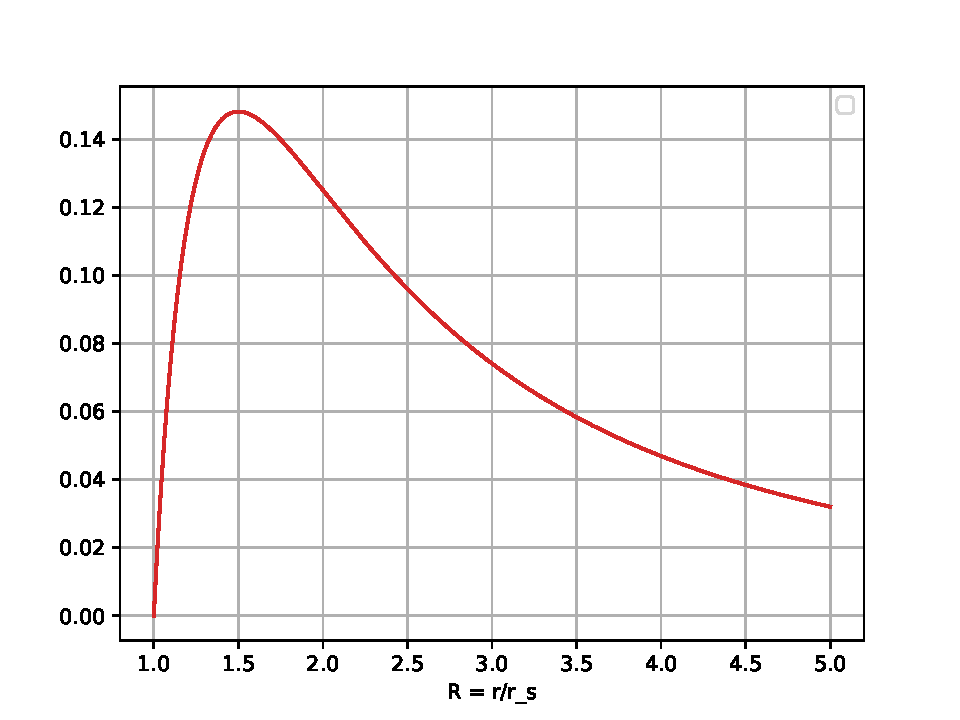
\includegraphics[width=0.7\textwidth]{figures/photon_effective_potential.pdf}
    \caption{Plot of the function \(R^{-2} - R^{-3}\).}
    \label{fig:effective-potential}
\end{figure}

The term \(b^{-2}\) is the maximum value which can be attained by the LHS: we can call it the total energy, the kinetic and potential contributions must add up to it. 
Also, the kinetic term is always positive. 
So, if the total energy is less than the maximum of the potential, the photon is constrained to stay on either side of the potential barrier around \(R = 3/2\). The potential there equals 
%
\begin{align}
  V(3/2) = (2GM)^{-2} \qty((3/2)^{-2} - (3/2)^{-3}) 
  = \frac{4/27}{(2GM)^2} = \frac{1}{27 (GM)^2}
\,,
\end{align} 
%
so the condition of the photon being above the potential barrier is 
%
\begin{align}
  E _{\text{tot}} &> V _{\text{max}}  \\
  \frac{e^2}{l^2} &> \frac{1}{27 G^2M^2}  \\
  \frac{l^2}{e ^2} &< 27G^2M^2
\,,
\end{align}
%
and under this condition, if the photon initially has positive \(\dv*{r}{\lambda }\) it will remain as such, since everything is continuous and (if the strict inequality is satisfied) we can never have \(\dv*{r}{\lambda }=0\). 

If instead we had \(l^2/e^2 < 27G^2M^2\) and the photon was initially travelling away from the black hole, there would come a point for which \(\dv*{r}{\lambda }\) would equal zero, and then it would become negative, since the photon could not go away from the center anymore. 

This can be understood graphically by drawing horizontal lines of constant total energy in the potential diagram. 

\subsubsection{A basis for a stationary observer}

If our observer's coordinates are \((t, r_{*}, \pi /2 , \varphi_{*} )\), that is, it is at rest with respect to our spatial coordinates but it is not following geodesic motion, then it will have nonzero 4-acceleration. So, since we know that velocity and acceleration are orthogonal, we can form our coordinate system as \((u^{\mu }, a^{\mu } / \sqrt{ a^{\rho } a_{\rho }}, e_{\theta }, e_{\varphi })\), where the angular basis vectors are simply normalized vectors in the \(\theta \) and \(\varphi \) directions.

This method has the advantage of being easily generalizable to find a comoving basis for any non-geodesic motion of our observer. 

Their 4-velocity must be normalized so that \(u^{\mu } u_{\mu }= -1\): so 
%
\begin{align}
  u^{\mu } = \left[\begin{array}{c}
  \dv{t}{\tau } \\ 
  0 \\ 
  0 \\ 
  0
  \end{array}\right]
  = 
  \left[\begin{array}{c}
  1/\sqrt{1 - \frac{2GM}{r}} \\ 
  0 \\ 
  0 \\ 
  0
  \end{array}\right]
\,,
\end{align}
%
then we can compute the 4-acceleration: it will be 
%
\begin{align}
  a^{\mu } &= u^{\nu } \nabla_{\nu } u^{\mu }
  = u^{\nu } \qty(\partial_{\nu } u^{\mu } + \Gamma^{\mu }_{\nu \rho } u^{\rho })  \\
  &= \frac{1}{\sqrt{1 - \frac{2GM}{r}}} \qty(\cancelto{}{\partial_{t} u^{\mu }} + \Gamma^{\mu }_{tt} u^{t})  \\
  &= \frac{1}{\sqrt{1-\frac{2GM}{r}}}
  \frac{1}{\sqrt{1-\frac{2GM}{r}}} \frac{A'}{2B} \delta^{\mu }_{r}
\,,
\end{align}
%
where \(A = 1/B = (1 - 2GM/r)\) are the coefficients of the Schwarzschild metric, with respect to which the Christoffel symbols are expressed in \eqref{eq:schwarzschild-christoffel}. 
The \(\delta^{\mu }_{r}\) signifies that the only component which survives is the radial one.
The two square root terms simplify the \(B\), so we get that the only nonzero component of the 4-acceleration is:
%
\begin{align}
  a^{r} = \frac{A^{\prime }}{2} =
  \frac{1}{2} \dv{}{r} \qty(1 - \frac{2GM}{r})
  = \frac{GM}{r^2}
\,.
\end{align}
%
The actual value of this component is not actually useful to us --- except as an illustration of the equivalence principle: it is the precise value of the Newtonian pseudo-force of acceleration --- since we need a normalized basis. Therefore, we will use a vector parallel to \(a^{\mu }\) but of length defined by the normalization \(e_{r} \cdot e_{r} = 1\). So, we get for our basis: 
%
\begin{align}
  \begin{cases}
    (e_{t})^{\mu } = u^{\mu } = \left[\begin{array}{cccc}
    (1-2GM/r)^{-1/2}, & 0, & 0, & 0
  \end{array}\right]^{\top} \\ 
    (e_{r})^{\mu } = a^{\mu } / \sqrt{a_{\rho } a^{\rho }}
  = \left[\begin{array}{cccc}
    0, & (1-2GM/r)^{1/2}, & 0, & 0
  \end{array}\right]^{\top}  \\
  (e_{\theta })^{\mu } = \left[\begin{array}{cccc}
  0, & 0, & 1/r, & 0
  \end{array}\right]^{\top} \\
  (e_{\varphi })^{\mu } = \left[\begin{array}{cccc}
  0, & 0, & 0, & 1/(r \sin \theta )
  \end{array}\right]^{\top}
\end{cases} 
\,,
\end{align}
%
where the last vector is written for a generic angle \(\theta \), but the sine is equal to one if \(\theta = \pi /2\). 
This basis satisfies the property \(e_{\alpha } \cdot e_{\beta } = \eta_{\alpha \beta }\). 

We will denote vectors written with respect to this basis with a subscript \(c\). 

\subsubsection{Critical angle of launch}

In the flat frame, the 4-velocity of the photon launched at \(\theta = \pi /2\) looks like: 
%
\begin{align}
  u^{\mu } _{\text{ph}} = \left[\begin{array}{c}
  1 \\ 
  \cos \psi  \\ 
  0 \\ 
  \sin \psi 
  \end{array}\right]_c
\,,
\end{align}
%
which means that in the Schwarzschild frame it looks like 
%
\begin{align}
  u^{\mu }_{\text{ph}} = \left[\begin{array}{c}
  \frac{1}{\sqrt{1-\frac{2GM}{r}}} \\ 
  \cos \psi \sqrt{1 - \frac{2GM}{r}} \\ 
  0 \\ 
  \frac{\sin \psi}{r} 
  \end{array}\right]
\,.
\end{align}

This means that the parameter \(l = r \sin \psi \), while \(e = \sqrt{1-2GM/r}\). 

The inequality to satisfy for the photon to be able to escape is: 
%
\begin{align}
  \qty[\frac{e^2}{l^2}]_{r_{*}} \geq \frac{1}{27G^2M^2}
\,,
\end{align}
%
which translates to 
%
\begin{align}
  \frac{1 - \frac{2GM}{r_{*}}}{r_{*}^2 \sin^2 \psi } \geq \frac{1}{27G^2M^2}
\,,
\end{align}
%
or 
%
\begin{align}
  r_{*}^2 \sin^2 \psi \leq 27G^2M^2 \qty(1 - 2GM/r_{*}) 
  \,,
\end{align}
%
\begin{figure}[ht]
  \centering
  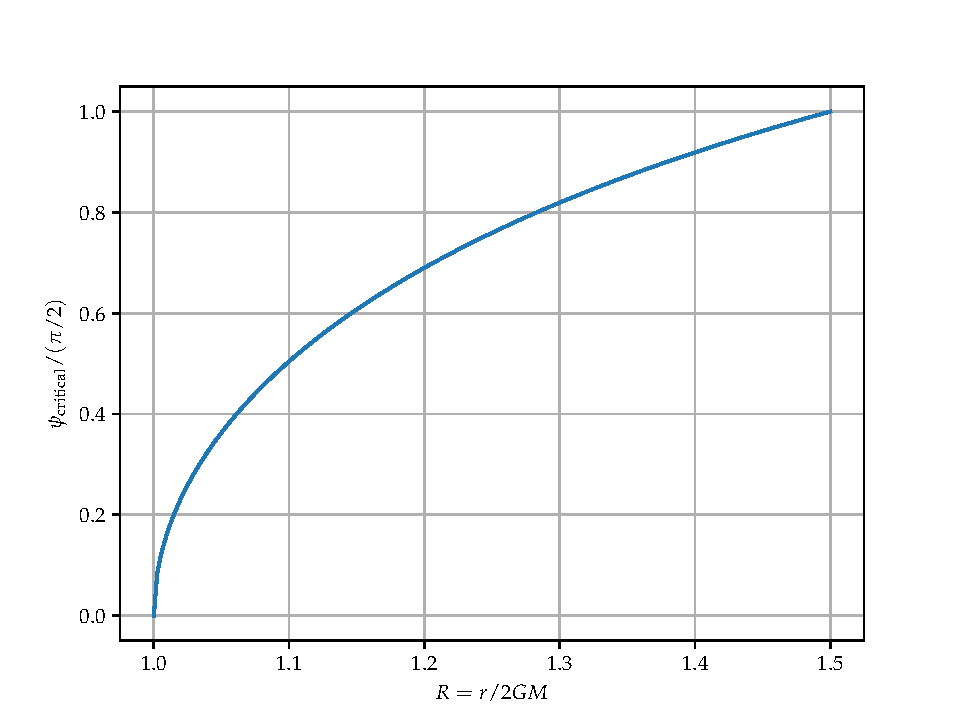
\includegraphics[width=0.7\textwidth]{figures/critical_psi.pdf}
  \caption{Critical angle \(\psi \) in terms of the adimensional radial coordinate \(R = r/ 2GM\).}
  \label{fig:critical-psi}
\end{figure}
%
which once again can be expressed in terms of the adimensional radial coordinate \(R = r/2GM\): we find 
%
\begin{align}
  \sin^2 \psi \leq \frac{27}{4 R_{*}^2} \qty(1 - \frac{1}{R_{*}})
  \,,
\end{align}
%
so the critical angle can be computed by making the relation explicitly in terms of \(\psi \), which gives the plot shown in figure \ref{fig:critical-psi}, for the equation 
%
\begin{align}
  \psi = \arcsin \sqrt{\frac{27}{4 R_{*}^2} \qty(1 - \frac{1}{R_{*}})}
\,.
\end{align}
%

So, as we move closer to the horizon, the range of angles at which we can throw our photon and still have it escape decreases, until finally we can only throw it straight forward otherwise it will fall back in. After \(r = 2GM\), not even that is enough.  

All communication with the outside world is lost. 

\subsection{Light motion in a Schwarzschild geometry}

\subsubsection{Equation of motion}

This was done during the lectures, but I will recall it here. 

We start from the equation of motion of a photon, a reframing of \(u^2=0\): 
%
\begin{align}
  \frac{1}{l^2} \qty(\dv{r}{\lambda })^2 + V _{\text{eff}} (r) = \frac{1}{b^2} = \frac{e^2}{l^2}
\,.
\end{align}

We want to write this as a differential equation for the radius in terms of the angle \(\varphi \): so, we use the expression of the first integral 
%
\begin{align}
  l = \dv{\varphi }{\lambda } r^2 \implies \dv{\varphi }{\lambda } = \frac{l}{r^2} \implies \dv{}{\lambda } = \frac{l}{r^2} \dv{}{\varphi }
\,.
\end{align}
%

So, we can rewrite 
%
\begin{align}
  \qty(\dv{r}{\lambda })^2= \frac{l^2}{r^{4}} \qty(\dv{r}{\varphi })^2
\,,
\end{align}
%
which allows us to write the equation as 
%
\begin{align}
  \frac{1}{r^{4}} \qty(\dv{r}{\varphi })^2 + V _{\text{eff}}(r) = \frac{1}{b^2}
\,,
\end{align}
%
since the \(l^2\) simplifies. 

Now, notice that if we define \(u = 1/r\) we find
%
\begin{align}
  \dv{u}{\varphi } = - \frac{1}{r^2} \dv{r}{\varphi }
\,,
\end{align}
%
which conveniently simplifies the \(r^{-4}\): expressing everything with respect to \(u\) we get 
%
\begin{align}
  \qty(\dv{u}{\varphi })^2 +  \qty(u^2-2GMu^3) = \frac{1}{b^2}
\,.
\end{align}

Now, we just need to differentiate everything to eliminate the constant term and find 
%
\begin{align}
  2 u' u'' + 2 u u' - 6 GM u^2 u' = 0
\,,
\end{align}
%
where we denoted derivatives with respect to \(\varphi \) with primes.
One solution is \(u'=0\): a circular orbit, which we are not interested in now (and which is unstable\dots).

Otherwise, we can simplify a factor \(2 u'\): we find 
%
\begin{align}
  u'' + u = 3 GMu^2
\,
\end{align}
%
as we wanted to show. 

\subsubsection{Zero black hole mass solution}

If \(M=0\), our diffential equation is simply \(u''+u=0\), a harmonic oscillator.
Our boundary condition is \(r (\varphi = 0, \pi ) \rightarrow \infty \), which means \(u \rightarrow 0\) in those cases. 

Also, one can geometrically see that at any radius \(\sin \varphi = b/r\) where \(b\) is the impact parameter.
Therefore, \(bu = \sin \varphi \) or \(u = \sin(\varphi ) / b \). This actually is already a solution to our differential equation! 

We are giving two boundary conditions, therefore the solution \(u = \sin(\varphi ) / b \) is unique. 

\subsubsection{Small mass deflection}

We now insert a mass \(M\), and consider a solution which is a perturbation to the sinusoidal one: our proposed solution is \(u = b^{-1} (\sin \varphi + w)\), and we will only look at the first order in \(w\). Substituting into \(u'' + u = 3GM u^2\) we get 
%
\begin{align}
  - \sin \varphi + w'' + \sin \varphi + w = \frac{3GM}{b} \qty(\sin^2 \varphi + \cancelto{}{2w  \sin \varphi} + \cancelto{}{w^2})
\,,
\end{align}
%
where we kept only terms which are of first order in either \(GM\) or \(w\), since both are small relative to the scale of the problem. Also, we simplified a common factor of \(b\).
So the differential equation for \(w\) is 
%
\begin{align}
  w'' + w = \frac{3GM}{b} \sin^2 \varphi 
\,.
\end{align}

This can be solved with an \emph{ansatz} in the form \(w = A + B \sin^2\varphi\).
Its derivatives are \(w' = 2B \sin \varphi \cos \varphi = B \sin(2\varphi )\), and \(w'' = 2B \cos(2 \varphi )= 2 B \qty(1 - 2\sin^2\varphi )\). 

Plugging this in we find 
%
\begin{align}
  2 B (1 - 2 \sin^2 \varphi) + A + B \sin^2 \varphi = \frac{3GM}{b} \sin^2 \varphi 
\,,
\end{align}
%
so equating the terms in \(\sin^2\varphi  \) and the constant ones we get 
%
\begin{align}
  \begin{cases}
    2B+A = 0 \\
    -3B = 3GMb^{-1}
  \end{cases}
\,,
\end{align}
%
so our perturbation is \(w = 2 GM b^{-1} (1- \sin^2 \varphi / 2)\), therefore the full solution is 
%
\begin{align}
  u(\varphi ) = \frac{1}{b} \qty(\sin \varphi + \frac{2GM}{b} \qty(1 - \frac{\sin^2 \varphi }{2}))
\,.
\end{align}
%

What follows is an alternative derivation, more complicated than plainly discarding the second-order \(\sin^2  \varphi  \) term and expanding the sine to first order, which gives \(\varphi \sim -2GM/b\) right away. I did it in this way mostly to check that it still works. 

We want to solve the equation of the particle coming in from radial infinity at an angle \(\varphi _{\text{in}}\), and leaving at an angle \(\varphi _{\text{out}}\) towards radial infinity. This means that we are seeking two solutions to \(r = \infty \implies u = 0\), respectively near \(\varphi = 0\) and \(\varphi = \pi \). This can be written as a second degree equation in terms of the variable \(x = \sin \varphi \), and the adimensionalized impact parameter \(b/ 2GM = d\), by which we multiply everything to get:  
%
\begin{align}
  x^2 - 2dx - 2 = 0
\,,
\end{align}
%
which can be solved as 
%
\begin{align}
  x =d \pm \sqrt{d^2 + 2}
  = d \qty(1 \pm \sqrt{1 + \frac{2}{d^2}})
\,,
\end{align}
%
so we have two solutions: one near \(x=0\), one near \(x=2d\). The second is meaningless, since \(d \gg 1 \) but \(x \leq 1\). Expanding around \(d = \infty\) we find: 
%
\begin{align}
  x = d \qty(1 - \qty(1 + \frac{1}{2} \frac{2}{d^2})) = -\frac{d}{2}  \frac{2}{d^2} = -\frac{1}{d} = - \frac{2GM}{b} = \sin \varphi 
\,. 
\end{align}
%

So, we want solutions to this near \(\varphi = 0\) and \(\varphi = \pi \), and we are working up to first order in \(\varphi \). Then, we have 
%
\begin{align}
  \varphi _{\text{in}} = - \arcsin \qty(\frac{2GM}{b}) 
  \sim - \frac{2GM}{b}
\,
\end{align}
%
and  
%
\begin{align}
  \varphi _{\text{out}}  = \pi + \arcsin \qty( \frac{2GM}{b}) \sim \pi + \frac{2GM}{b}
\,.
\end{align}
%
The deflection can be calculated by assuming \( \varphi _{\text{out}} - \varphi _{\text{in}} = \pi + \delta \varphi \), which gives 
%
\begin{align}
  \delta \varphi \approx \frac{4GM}{b}
\,.
\end{align}
%

\subsubsection{Newtonian prediciton and Eddington observations (complement)}

The Newtonian prediction, which is computed using the Keplerian formula for eccentricity (and, notably, simplifying the ``mass'' of a light particle) is instead:\footnote{\url{https://arxiv.org/pdf/physics/0508030.pdf}}
%
\begin{align}
  \delta \varphi \approx \frac{2GM}{b}
\,.
\end{align}

During the solar eclipse of 1919, Sir Eddington\footnote{\url{https://royalsocietypublishing.org/doi/abs/10.1098/rsta.1920.0009}} made two observations: one gave 
%
\begin{align}
  \delta \varphi = \qty(\SI{4.5(3)}{}) \frac{GM}{b}
\,,
\end{align}
%
and another gave 
%
\begin{align}
  \delta \varphi = \qty(\SI{3.7(7)}{}) \frac{GM}{b}
\,.
\end{align}
%

\subsection{Orbit at 7GM}

\subsubsection{Orbital radius}

The radius of a \(7G M_{\odot}\) orbit is equal to 
%
\begin{align}
  7GM_{\odot}/c^2 \approx\\
  7 \times \SI{6.67e-11}{kg m^{3} s^{-2}} \times \SI{2e30}{kg} \times \qty(\SI{3e8}{ms^{-1}})^{-2} \approx \\
  \approx \SI{1.0e4}{m}
\,,
\end{align}
%
or around \SI{10}{km}. 

\subsubsection{Proper period}

The equation governing a circular orbit around a BH can be derived from the normalization of the 4-velocity \(u \cdot u = -1\): in terms of \(u = 1/r\) it is 
%
\begin{align}
  u_c = \frac{GM}{l^2} + 3 GM u_c^2
\,,
\end{align}
%
and in our case we know that \(u_c = 1/7GM\), substituting in we find 
%
\begin{align}
  \frac{1}{7GM} = \frac{GM}{l^2} + \frac{3GM}{49 (GM)^2}
\,,
\end{align}
%
or 
%
\begin{align}
  l^2 = (GM)^2 \qty(\frac{1}{7} - \frac{3}{49})^{-1}
  = 7 (GM)^2 \qty(1 - \frac{3}{7})^{-1} = \frac{49}{4} (GM)^2
\,, 
\end{align}
%
so \(l = 7GM/2\). Now, recall the definition of this first integral: 
%
\begin{align}
  l = \dv{\varphi }{\tau } r^2
\,,
\end{align}
%
into which we can substitute the expression we found: 
%
\begin{align}
  \frac{7GM}{2} (7GM)^{-2} = \frac{1}{14GM} =  \dv{\varphi }{\tau } = \omega_{\text{proper}}
\,,
\end{align}
%
which gives us the angular velocity as measured by the orbiting observer. We actually have it in units of $1/\SI{}{m^3 s^{-2}}$, so we will need to multiply by \(c^3\) to get inverse seconds.

This gives us a pulsation of 
%
\begin{align}
  \omega _{\text{proper}} = \frac{c^3}{14GM_{\odot}} \approx 
  \SI{1.44e5}{rad/s}
\,,
\end{align}
%
which corresponds to a period of 
%
\begin{align}
  T _{\text{proper}} = \frac{2\pi}{\omega _{\text{proper}}} \approx \SI{4.36e-4}{s} = \SI{436}{\micro s}
\,.
\end{align}

\subsubsection{Period at infinity}

Now, to compute the period for an observer at infinity: from the regular equation of motion of a massive observer we have 
%
\begin{align}
  \frac{e^2-1}{2} = \frac{1}{2} \qty(\dv{r}{\tau })^2+ \underbrace{\qty(-\frac{GM}{r} + \frac{l^2}{2r^2} - \frac{GMl^2}{r^3})}_{V _{\text{eff}}}
\,,
\end{align}
%
but since the orbit is circular \(r\) is constant so the derivative vanishes, and we can substitute in our expressions for \(r\) and \(l\) to find out what \(e\) is: we get 
%
\begin{align}
  \frac{e^2-1}{2} &= - \frac{GM}{7GM} + \frac{(7GM/2)^2}{2\times (7GM)^2} - \frac{GM (7GM/2)^2}{(7GM)^3}  \\
&= - \frac{1}{7}+ \qty(\frac{7}{2})^2 \frac{1}{2\times 7^2} - \qty(\frac{7}{2})^2 \frac{1}{7^3}  \\
&= -\frac{3}{56}
\,,
\end{align}
%
therefore \(e = 5 \sqrt{7} / 14\). Now recall the definition of \(e\): 
%
\begin{align}
  e = \dv{t}{\tau } \qty(1 - \frac{2GM}{r}) 
\,,
\end{align}
%
so 
%
\begin{align}
  \frac{T_{ \infty }}{T _{\text{proper}}} = 
  \dv{t}{\tau } = \frac{5 \sqrt{7}}{14} \qty(1 - \frac{2GM}{7GM})^{-1} = \frac{\sqrt{7}}{2} \approx 1.323 
\,,
\end{align}
%
therefore the period as measured by the outside observer is 
%
\begin{align}
  T_{ \infty } \approx \SI{577}{\micro s}
\,.
\end{align}
%

Do note that this is \emph{not} the same as plainly applying the gravitational redshift formula as \(T_1 / T_2 = \sqrt{ g_{tt}^{1}/ g_{tt}^{2}}\): that gives a smaller ratio. The Doppler effects of the orbital speed do not average out over a period, it seems. 

\subsubsection{Proper acceleration}

The orbit is a geodesic, so a pointlike observer feels no acceleration. 

\subsubsection{Tidal acceleration (complement)}

A pointlike particle would feel no acceleration, however it would be quite unconfortable to be in that orbit if one happens not to be pointlike. 
As for the first part of the exercise, this is not in the exercise sheet, so do skip it if you are in a hurry. I think it is quite interesing though.

Let us compute the tidal effects on an extended observer. 

They are described by the equation 
%
\begin{align}
  \dv[2]{\xi^{\mu }}{\tau } = R^{\mu }_{\nu \rho \sigma } u^{\nu } u^{\rho } \xi^{\sigma }
\,,
\end{align}
%
where \(u^{\mu }\) is the 4-velocity of a geodesic, \(\xi^{ \mu } \) is a small deviation in starting position for the geodesic such that the geodesic starting from there almost has the same tangent vector. For now we assume it to be true, in the next section we give justification for it. 

We can restrict ourselves to radial geodesic deviation: then we only need to compute the \(R^{r}_{\nu \rho r}\) components of the Riemann tensor. 
I might do the full computation, but I found a source\footnote{\url{https://physics.stackexchange.com/questions/295814/non-zero-components-of-the-riemann-tensor-of-the-schwarzschild-metric}} which gives the nonzero components: 
%
\begin{align}
  R^{r}_{ttr} &= \frac{2GM}{r^3} \qty(1 - \frac{2GM}{r}) \\
  R^{r}_{\theta \theta r} &= \frac{GM}{r} \\
  R^{r}_{\varphi \varphi r} &= \frac{G M \sin^2\theta}{r} 
\,,
\end{align}
%
and since the orbital motion is assumed to happen on the \(\theta = \pi /2\) plane, the formula simplifies to 
%
\begin{align}
  \dv[2]{\xi^{r}}{\tau } &= R^{r}_{ttr} u^{t} u^{t} \xi^{r} 
  + R^{r }_{\varphi \varphi r} u^{\varphi } u^{\varphi } \xi^{r}  \\
  &= \qty(\frac{e^2}{(1-2GM/r)^2} \frac{2GM}{r^{3}}\qty(1 - \frac{2GM}{r}) +  \frac{l^2}{r^{4}} \frac{GM}{r}) \xi^{r}  \\
  &= \qty(\frac{e^2}{1-2GM/r} + \frac{l^2}{r^2} ) \frac{2GM}{r^3} \xi^{r}
\,,
\end{align}
%
which holds in general: in our specific case, at \(r = 7GM \) we find 
%
\begin{align}
  \dv[2]{\xi^{r}}{\tau } &= \qty(\frac{7}{5} \qty(\frac{5 \sqrt{7}}{14})^2 + \qty(\frac{7GM/2}{7GM})^2 ) \frac{2GM}{(7GM)^3}  \xi^{r}  \\
  &= \frac{3}{343} \frac{1}{(GM)^2} \xi^{r}
\,,
\end{align}
%
so the object multiplying \(\xi^{r}\), in units of inverse square seconds, is 
%
\begin{align}
  \frac{3}{343} \frac{c^{6}}{(GM)^2} \approx \SI{356e6}{s^{-2}}
  \approx \qty(\SI{18.9}{kHz})^2
\,. 
\end{align}

The acceleration which would be experienced from one side of the other of a meter-long observer would then be of around \SI{36}{M}\(g\). 

\subsubsection{A proof for the geodesic deviation formula (complement)}

The starting separation between geodesics is not, properly speaking, a \emph{vector} since it does not belong to the tangent space, however we can be sloppy and approximate it as a tangent vector.
Then it is a fact from differential geometry that under an assumption of vanishing torsion (which we always make anyways in GR) and if the vector fields \(u^{\mu }\) and \(\xi^{\mu }\) commute the following holds: 
%
\begin{align} \label{eq:lie-bracket-commutation}
  \xi^{\mu } \nabla_{\mu } u^{\nu } = u^{\mu } \nabla_{\mu } \xi^{\nu }
\,.
\end{align}

\todo[inline]{We can have commuting vector fields if we choose a basis; can we say that we derive the formula for geodesic deviation for the basis vectors and extend by linearity?}

So, we want to see by how much the two initially-close geodesics diverge: in order to do this, we compute the second derivative of \(\xi^{\mu }\) with respect to proper time: recall that the derivative with respect to proper time is also the Lie derivative along the 4-velocity: \(\dv*{}{t} = u^{\mu } \nabla_{\mu }\). 

So, this second derivative looks like 
%
\begin{align}
  \dv[2]{\xi^{ \mu } }{\tau } = u^{\alpha } \nabla_{\alpha } \qty(u^{\beta } \nabla_{\beta } \xi^{\mu })
  = u^{\alpha } \nabla_{\alpha } \qty( \xi^{\beta }\nabla_{\beta } u^{\mu } )
\,
\end{align}
%
by the formula shown above. Now, we can apply the Leibniz rule: we find 
%
\begin{align}
  \dv[2]{\xi^{\mu }}{\tau } = u^{\alpha } \qty( \qty(\nabla_{\alpha } \xi^{\beta }) \qty(\nabla_{\beta } u^{\mu })  
  + \xi^{\beta } \nabla_{\alpha } \nabla_{\beta } u^{\mu } )
\,,
\end{align}
%
and using the fact that\footnote{A trick for remembering this: it would be intuitive to just write the lower indices as \(\alpha \beta \gamma \), but the last two are antisymmetric and must correspond to the antisymmetrization of the covariant derivatives in the LHS.} \([\nabla_{\alpha }, \nabla_{\beta }] V^{\mu } = R^{\mu }_{ \gamma \alpha \beta  } V^{\gamma }\) we can commute the covariant derivatives by inserting a Riemann tensor: we get 
%
\begin{align}
  \dv[2]{\xi^{\mu }}{\tau } = u^{\alpha } \qty( \qty(\nabla_{\alpha } \xi^{\beta }) \qty(\nabla_{\beta } u^{\mu })  
  + \xi^{\beta } \nabla_{\beta }\nabla_{\alpha } u^{\mu }
  + \xi^{\beta } R^{\mu }_{ \gamma \alpha \beta  } u^{\gamma } )
\,,
\end{align}
%
and now we have gotten the term which will remain in the end: let us bring it to the front, then we will show that the rest of the expression is null. We get 
%
\begin{align}
  \dv[2]{\xi^{\mu }}{\tau } =
  R^{\mu }_{ \gamma \alpha \beta  } u^{\gamma } u^{\alpha } \xi^{\beta } 
  + 
  u^{\alpha } \qty( \qty(\nabla_{\alpha } \xi^{\beta }) \qty(\nabla_{\beta } u^{\mu })  
  + \xi^{\beta } \nabla_{\beta }\nabla_{\alpha } u^{\mu } )
\,.
\end{align}
%

To show that the rest of the expression is zero, the thing to remember is that we want to use the fact that our curve is a geodesic, which is expressed as 
%
\begin{align}
  u^{\alpha } \nabla_{\alpha } u^{\mu } = \dv{}{\tau } u^{\mu } = 0 
\,,
\end{align}
%
so we apply the Leibniz rule backward, to find: 
%
\begin{align}
  & u^{\alpha } \qty( \qty(\nabla_{\alpha } \xi^{\beta }) \qty(\nabla_{\beta } u^{\mu })  
  + \xi^{\beta } \nabla_{\beta }\nabla_{\alpha } u^{\mu } )= \\
  =& u^{\alpha } \qty(\nabla_{\alpha } \xi^{\beta }) \qty(\nabla_{\beta } u^{\mu }) 
  + \xi^{\beta } \nabla_{ \beta } \qty( \cancelto{}{u^{\alpha } \nabla_{\alpha } u^{\mu }}) 
  - \xi^{\beta } \qty(\nabla_{\alpha } u^{\mu } ) (\nabla_{\beta } u^{\alpha })  \\
  =& u^{\alpha } \qty(\nabla_{\alpha } \xi^{\beta }) \qty(\nabla_{\beta } u^{\mu }) 
  - u^{\beta } \nabla_{\beta }\xi^{\alpha } ( \nabla_{\alpha } u^{\mu }) = 0
\,,
\end{align}
%
where in the last step we applied again the commutation relation \eqref{eq:lie-bracket-commutation}, and finally recognised that the terms were equal up to a relabeling of indices. 

\end{document}
